% !TEX spellcheck = en_US
% !TEX spellcheck = LaTeX
\documentclass[a4paper,10pt,english]{article}
\usepackage{%
	amsfonts,%
	amsmath,%	
	etex,%
	amssymb,%
	amsthm,%
	babel,%
	bbm,%
	%biblatex,%
	caption,%
	centernot,%
	color,%
	enumerate,%
	epsfig,%
	epstopdf,%
	geometry,%
	graphicx,%
	hyperref,%
	latexsym,%
	mathtools,%
	multicol,%
	pgf,%
	pgfplots,%
	pgfplotstable,%
	pgfpages,%
	proof,%
	psfrag,%
	subfigure,%	
	tikz,%
	ulem,%
	url%
}	

\usepackage[mathscr]{eucal}
\usepgflibrary{shapes}
\usetikzlibrary{%
  arrows,%
	backgrounds,%
	chains,%
	decorations.pathmorphing,% /pgf/decoration/random steps | erste Graphik
	decorations.text,%
	matrix,%
  	positioning,% wg. " of "
  	fit,%
	patterns,%
  	petri,%
	plotmarks,%
  	scopes,%
	shadows,%
  	shapes.misc,% wg. rounded rectangle
  	shapes.arrows,%
	shapes.callouts,%
  	shapes%
}

\theoremstyle{plain}
\newtheorem{thm}{Theorem}[section]
\newtheorem{lem}[thm]{Lemma}
\newtheorem{prop}[thm]{Proposition}
\newtheorem{cor}[thm]{Corollary}

\theoremstyle{definition}
\newtheorem{defn}[thm]{Definition}
\newtheorem{conj}[thm]{Conjecture}
\newtheorem{exmp}[thm]{Example}
\newtheorem{assum}[thm]{Assumptions}
\newtheorem{axiom}[thm]{Axiom}

\theoremstyle{remark}
\newtheorem{rem}{Remark}
\newtheorem{note}{Note}

\newcommand{\norm}[1]{\left\lVert#1\right\rVert}
\newcommand{\indep}{\!\perp\!\!\!\perp}
\DeclarePairedDelimiter\abs{\lvert}{\rvert}%
%\DeclarePairedDelimiter\norm{\lVert}{\rVert}%
\newcommand{\tr}{\operatorname{tr}}
\newcommand{\R}{\mathbb{R}}
\newcommand{\Q}{\mathbb{Q}}
\newcommand{\N}{\mathbb{N}}
\newcommand{\E}{\mathbb{E}}
\newcommand{\Z}{\mathbb{Z}}
\newcommand{\B}{\mathscr{B}}
\newcommand{\C}{\mathcal{C}}
\newcommand{\T}{\mathscr{T}}
\newcommand{\F}{\mathcal{F}}
\newcommand{\G}{\mathcal{G}}
%\newcommand{\ba}{\begin{align*}}
%\newcommand{\ea}{\end{align*}}

\makeatletter
\def\th@plain{%
  \thm@notefont{}% same as heading font
  \itshape % body font
}
\def\th@definition{%
  \thm@notefont{}% same as heading font
  \normalfont % body font
}
\makeatother
\date{}
\title{Lecture 03: Properties of Poisson Process}
\author{}

\begin{document}
\maketitle

\section{Conditional Distribution of Arrivals}
\begin{prop}\label{Prop:SIIPoisson}
Let $\{N(t), t\geqslant 0\}$ be a Poisson process with $\{A_i \subseteq \R_+: i \in [n]\}$ a set of finite disjoint intervals with $B = \cup_{i \in [n]}A_i$, and $\{k_i \in \N : i \in [n]\}$ and $k = \sum_{i \in [n]}k_i$. Then, we have 
\begin{align*}
\Pr\bigcap_{i \in [n]}\{N_{A_i} = k_i | N(B) = k\} &= k!\prod_{i \in [n]}\frac{1}{k_i!}\left(\frac{|A_i|}{|B|}\right)^{k_i}.
\end{align*}
\end{prop}
\begin{proof}
It follows from the stationary independent increment property of Poisson processes that
\begin{align*}
\Pr\bigcap_{i \in [n]}\{N_{A_i} = k_i | N(B) = k\} &= \frac{\Pr\bigcap_{i \in [n]}\{N_{A_i} = k_i\}}{\Pr\{N_B = k\}} = \frac{1}{\Pr\{N_B = k\}}\prod_{i \in [n]}\Pr\{N_{A_i} = k_i\}.
\end{align*}
\end{proof}

\begin{prop} 
For a Poisson process $\{N(t), t\geqslant 0\}$, distribution of first arrival instant $S_1$ conditioned on $\{N(t)=1\}$ is uniform between $[0,t)$.
\end{prop}
\begin{proof} If $N(t) = 1$, then we know that conditional distribution of $S_1$ is supported on $[0,t)$. By Proposition~\ref{Prop:SIIPoisson}, we see that
\begin{align*}
\Pr\{S_1 \leq s | N(t) = 1\} &= \Pr\{ N(s) = 1, N(t-s) = 0 | N(t) = 1\}1_{\{s < t\}} = \frac{s}{t}1_{\{s < t\}}.
\end{align*}
\end{proof}
\begin{proof}[Alternative proof]
For any $0 \leq u < t$, we can write $\{S_1 = u, N(t) = 1\}$ as intersection of two independent events, %as follows
\begin{align*}
\{S_1 = u, N(t) = 1\} \iff \{S_1 = u\}\cap\{X_2 > t - u\}.
\end{align*}
Therefore, integrating LHS with respect to $u$ in interval $[0,s]$ for $s < t$, we obtain
\begin{align*}
\Pr\{S_1 \leq s, N(t) = 1\} = \int_{0}^{s}du \lambda \exp(-\lambda u)\exp(-\lambda (t-u)) = s\lambda\exp(-\lambda t).
\end{align*}
Since $\Pr\{N(t) = 1\} = \lambda t \exp(-\lambda t)$, it follows that 
\begin{align*}
\Pr\{S_1 \leq s| N(t) = 1\} = \begin{cases}\frac{s}{t}, & s < t\\ 0, & s \geq t.\end{cases}.
\end{align*}
%\noindent For the  with rate $0<\lambda< \infty$, we would like to find the density.
%\begin{eqnarray*}
%% \nonumber to remove numbering (before each align)
  %P(S_{1}\mid N(t)=1), t>0 \\
  %P_{S_1}(S \mid N(t)=1) \\
  %P(s\leq S_{1} \leq s+h \mid N(t)=1)\\
   %&\approx& h P_{S_1}(S \mid N(t)=1 \\
  %P(s\leq S_{1}< s+h \mid N(t)=1)\\
   %&=& \frac{P(s\leq S_{1}< s+h,N(t)=1)}{P(N(t)=1)}\\
   %&=& \frac{\Pr\{s\leq S_{1}<s+h,X_{2}>t-(s+h))}{\lambda t e^{-\lambda t}} \\
   %&=& \frac{h \lambda e^{-\lambda h} e^{-\lambda (t-(s+h))}}{h{\lambda t} e^{-\lambda t}}.
   %\end{eqnarray*}
   %Take  $\lim _{h\rightarrow 0}\frac{1}{t}{e^{-\lambda h}} =\frac{1}{t}.$ Thus, the conditional density is the density of a uniform random variable distributed over the interval $[0,t].$ 
\end{proof}
%This property of Poisson process can be generalized for any set of arrival instants.
\begin{prop}%[Conditional Distribution of Arrival Instants] 
For a Poisson process $\{N(t), t\geqslant 0\}$, joint distribution of arrival instant $\{S_1, \ldots, S_n\}$ conditioned on $\{N(t)=n\}$ is identical to joint distribution of order statistics of $n$ \emph{iid} uniformly distributed random variables between $[0,t]$.
\end{prop}
\begin{proof} Let $\{ s_0 = 0 < s_1 < s_2 <\ldots < s_n < t \}$ be a finite sequence of non-negative increasing numbers between $0$ and $t$. Then, by Proposition~\ref{Prop:SIIPoisson}, we get
\begin{align*}
\Pr\bigcap_{i \in [n]}\{S_i \leq s_i | N(t) = n\} &= \Pr\bigcap_{i \in [n]}\{N((0, s_i]) \geq i | N(t) = n\}.
%\\&=\frac{1}{t^n}\sum_{a_1 + \ldots + a_n = n, a_i \geq i} \prod_{i \in [n]}\frac{(s_i - s_{i-1})^{a_i}}{a_i!}.
\end{align*}
\end{proof}
\begin{proof}[Alternative proof] Let $\{ s_i \in (0, t) : i \in [n]\}$ be a sequence of increasing numbers. If we denote $s_{0} = 0$, then we can write 
\begin{align*}
\bigcap_{i=1}^n\{S_i = s_i\}\cap\{N(t) = n\} \iff \bigcap_{i=1}^n\{X_i = s_i - s_{i-1}\}\cap\{X_{n+1} > t - s_n\}.
\end{align*}
Note that all the events on RHS are independent events. Therefore, it is easy to compute the joint distribution of $\{S_1,\ldots, S_n\}$, as 
\begin{align*}
\Pr\bigcap_{i=1}^n\{S_i \leq s_i\}\cap\{N(t) = n\} &= \int_{0}^{s_1}du_1\cdots\int_{0}^{s_n}du_n \prod_{i=1}^n\lambda \exp(-\lambda (u_i-u_{i-1})\exp(-\lambda (t-u_n))\\
&= \lambda^n\exp(-\lambda t)\prod_{i=1}^ns_i.
\end{align*}
Since $\Pr\{N(t) = n\} = \exp(-\lambda t)(\lambda t)^n/n! $, it follows that 
\begin{align*}
\Pr\{S_1 \leq s_1,\ldots, S_n\leq s_n | N(t) = n\} = 
\begin{cases}
n!\prod_{i=1}^n\frac{s_i}{t} & s < t\\ 
0 & s \geq t.
\end{cases}
\end{align*}
%\begin{eqnarray*}
%% \nonumber to remove numbering (before each align)
    %&\Pr\{s_{1}\leq S_{1}<s_{1}+h, s_{2}\leq S_{2}<s_{2}+h, ...s_{n}\leq S_{n}\leq s_{n}+h \mid N(t)=n]  \\
   %&=   \frac{\Pr\{s_{1}\leq S_{1}<s_{1}+h, s_{2}\leq S_{2}<s_{2}+h,...,s_{n}\leq S_{n}\leq s_{n}+h,N(t)=n]}{\Pr\{N(t)=n]} \\
   %&=  \frac{\Pr\{s_{1} \leq S_{1}<s_{1}+h_{1},s_{2}-s_{1}\leq X_{2}<s_{2}- (s_{1}+h),..., X_{n+1}> t-s_{n}]}{\Pr\{N(t)=n]} \\
   %&\stackrel{(a)}{=}  \frac{\Pr\{s_{1 \leq S_{1}<s_{1}+h}]\Pr\{s_{2}-s_{1}\leq X_{2}<s_{2}-s_{1}+h] \Pr\{X_{n+1}>t -s_{n}]}{\Pr\{N(t)=n]}\\
   %&=  \frac{\lambda h e^{-s_{1}\lambda}h \lambda e^{-(s_{2}-s_{1})\lambda},..., e^{-(t-s_{n})\lambda}}{(\lambda t)^{n}\frac{e^{-\lambda t}}{n!}} 
   %\end{eqnarray*}
   %\begin{eqnarray*}
    %\lim _{h\rightarrow 0} \frac{ \lambda h e^{-s_{1}\lambda}h \lambda e^{-(s_{2}-s_{1})\lambda},... e^{-(t-s_{n})\lambda}}{h^{n}(\lambda t)^{n}\frac{e^{-\lambda t}}{n!}}=\frac{n!}{t^{n}}.
%\end{eqnarray*}
%where (a) follows as $X_i$s are independent. 
Let $U_{1},\ldots,U_{n}$ are \emph{iid} Uniform random variables in $[0,t]$. Then, the order statistics  of $U_1 \ldots, U_n$ has an identical joint distribution to $n$ arrival instants conditioned on $\{N(t)=n\}$.\end{proof}

\section{Age and excess time}
\begin{defn} For a point process $\{N(t), t \geqslant 0\}$, we can define age process $\{A(t), t \geqslant 0\}$ and excess time process $\{Y(t), t \geqslant 0\}$ as 
\begin{xalignat*}{3}
&A(t) = t - S_{N(t)},&&Y(t) = S_{N(t)+1} - t.
\end{xalignat*}
\end{defn}
\begin{prop}
For a Poisson process with rate $\lambda$, the corresponding age and excess time are both exponentially distributed with rate $\lambda$ irrespective of time $t$.
\end{prop}
\begin{proof} Using stationary independent increment property of Poisson process, we can write complementary distribution of excess time process as 
\begin{align*}
\Pr\{Y(t) > y\} &= \sum_{n \in \N_0}\Pr\{Y(t) > y, N(t) = n\} = \sum_{n \in \N_0}\Pr\{N(t+y) - N(t) = 0, N(t) = n\}\\
&= \Pr\{N(y) = 0\}\sum_{n \in \N_0}\Pr\{N(t) = n\} = \Pr\{N(y) = 0\}.
\end{align*}
Similarly, we can write complementary distribution for the age process as
\begin{align*}
\Pr\{A(t) \geq x\} &= \sum_{n \in \N_0}\Pr\{A(t) \geq x, N(t) = n\} = \sum_{n \in \N_0}\Pr\{N(t) - N(t-x) = 0, N(t) = n\}\\
&= \sum_{n \in \N_0}\Pr\{N(t-x) = n\}\Pr\{N(x) = 0\} = \Pr\{N(x) = 0\}.
\end{align*}
\end{proof}
%We give some more properties of the Poisson process.
\section{Superposition and decomposition of Poisson processes}
\begin{thm}[Sum of Independent Poissons] Let $\{N_1(t), t \geqslant  0\}$ and $\{N_2(t), t \geqslant  0\}$ be two independent Poisson processes with rats $\lambda_{1}$ and $\lambda_{2}$ respectively. Then, the process $N(t)= N_{1}(t) +N_{2}(t)$ is Poisson with rate $\lambda_{1}+\lambda_{2}$.
\end{thm}
\begin{proof} We need to show that $\{N(t)\}$ has stationary independent increments, and 
\begin{align*}
	\Pr\{N(t)=n\}=   \exp(-(\lambda_{1}+\lambda_{2})t)\frac{(\lambda_{1}+\lambda_{2})^n t^n}{n!}.
\end{align*}
For two disjoint interval $(t_{1}, t_{2})$ and $(t_3,t_4)$, we can see that for both processes $N_{1}(t)$ and $N_2(t)$,  arrivals in $(t_{1}, t_{2})$ and $(t_3,t_{4})$ are independent. Therefore, $N(t)$ has independent increment property. Similarly, we can argue about the stationary increment property of $\{N(t)\}$. Further, we can write 
\begin{align*}
	\{N(t)=n\} = \bigcup_{k=0}^n\{\{N_1(t) = k\}\cap\{N_2(t) = n-k\}\}.
\end{align*}
Since $N_1(t)$ and $N_2(t)$ are independent, we can write
\begin{align*}
	\Pr\{N(t)=n\} &= \sum_{k=0}^n\exp(-\lambda_1t)\frac{(\lambda_1t)^k}{k!}\exp(-\lambda_2t)\frac{(\lambda_2t)^{n-k}}{(n-k)!},\\
	&= \frac{\exp(-(\lambda_1+\lambda_2)t)}{n!}\sum_{k=0}^n\binom{n}{k}(\lambda_1t)^k(\lambda_2t)^{n-k}.% = \exp(-(\lambda_1+\lambda_2)t)\frac{\{(\lambda_1+\lambda_2)t\}^n}{n!}.
\end{align*}
Result follows by recognizing that summand is just binomial expansion of $[(\lambda_1 + \lambda_2)t]^n$.
%\begin{eqnarray*}
%% \nonumber to remove numbering (before each align)
  %\Pr\{N(t)=n] &=& \Pr\{N_{1}(t)+ N_{2}(t)= n] \\
   %&=& \sum_{n1} P [N_{1}(t)=n_{1},N_{2}(t)= n-n_{1} ] \\
  %&=& \sum_{n_{1}}\frac{e^{-\lambda _{1}t}(\lambda_{1}t)^{n_{1}}}{n_{1}!}e^{-\lambda_{2}t}\frac{(\lambda_{2}t)^{(n-n_{1})}}{(n-n_{1})!} \\
   %&=&\sum_{n_{1} (\lambda _{2}t)} \frac{e^{-(\lambda_{1}+\lambda_{2})t} (\lambda_{1}t)^{n1}(\lambda_{2}t)^{-n_{1}}}{n_{1}! (n-n_{1})!} \\
   %&=& \frac{e^{-(\lambda_{1}+\lambda_{2})t}}{n!}\sum^{n}_{n_{1=0}}\left(\frac{\lambda_{1}}{\lambda_{2}}\right)^{n_{1}}\left(\frac{\lambda_{2}}{n_{1}!}\right)^{n}\frac{n!}{(n-n_{1})!} \\
   %&=&  \frac{e^{-(\lambda_{1}+\lambda_{2})t}}{n!}(\lambda_{1}+\lambda_{2})^{n}t^{n}
%\end{eqnarray*}
\end{proof}
\begin{rem}If independence condition is removed, the statement is not true.
\end{rem}
%\begin{figure}
%\centering
  %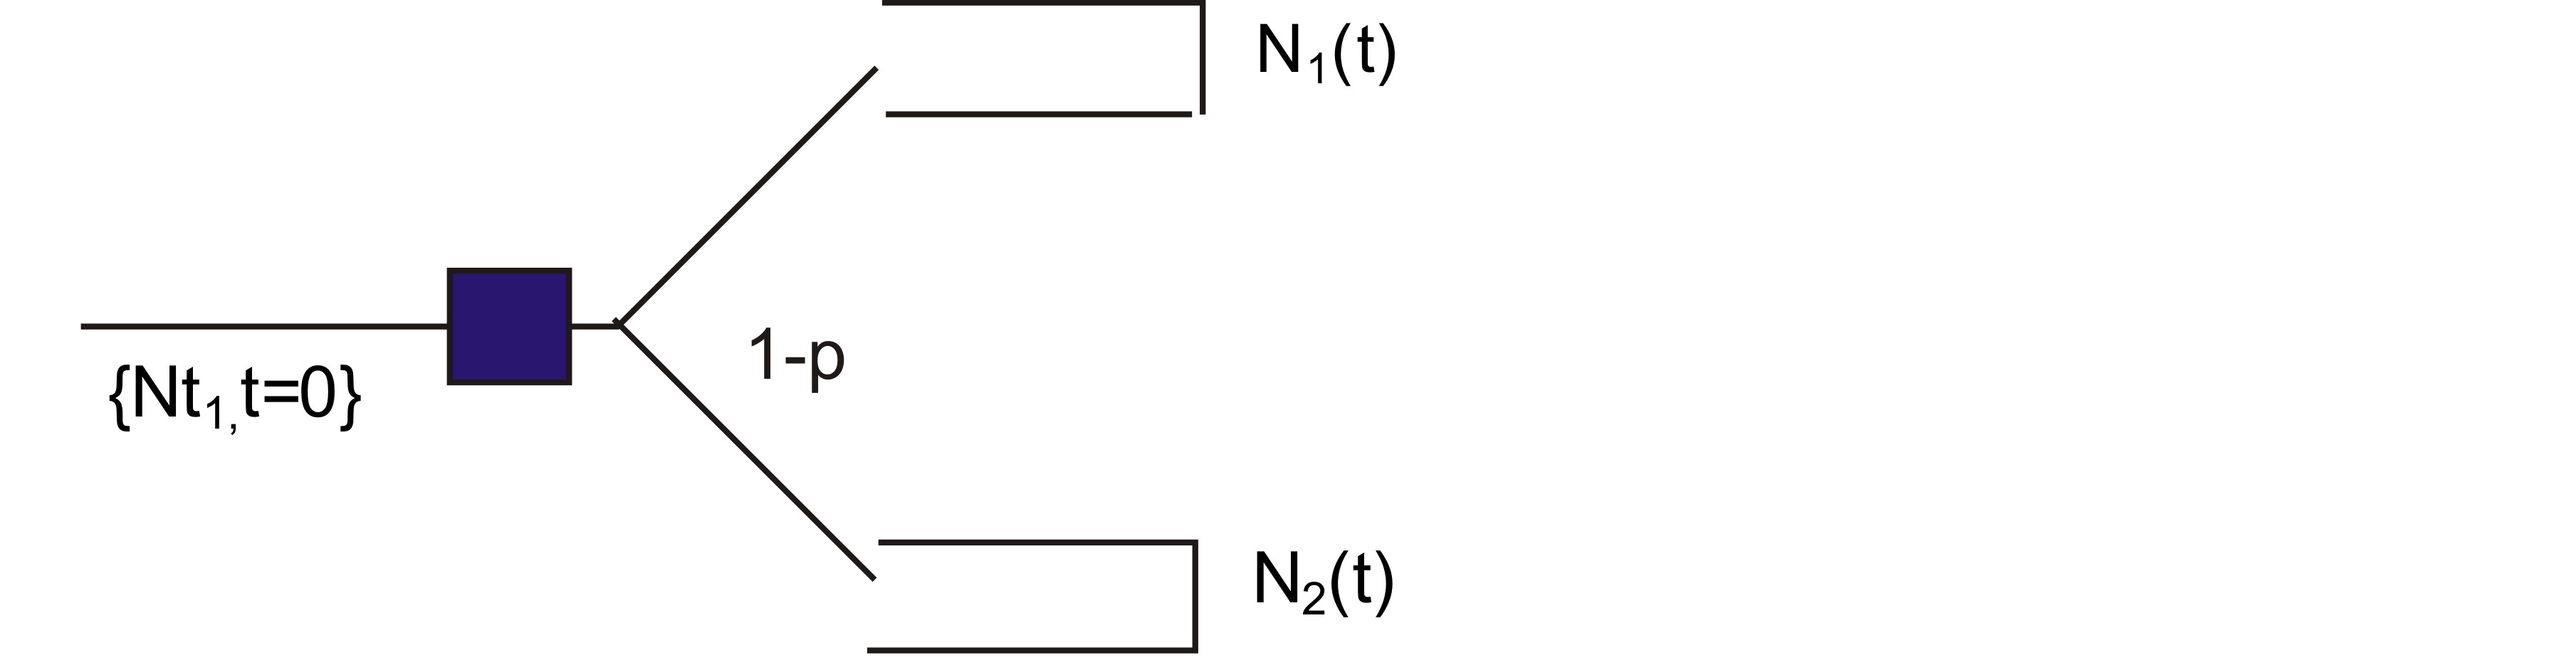
\includegraphics[width=5.0in]{Figures/comment.PNG}\\
 %% \caption{}\label{}
%\end{figure}
\begin{figure}[hhhh]
\center
  \begin{tikzpicture}
[node distance=1cm, draw=black, thick, >=stealth',
axes/.style=,
block/.style={rectangle, draw=black, rounded corners, inner sep=1pt, minimum height=0.8cm, minimum width=0.5cm},
queue/.style={rectangle, draw=white, rounded corners, inner sep=1pt, minimum height=0.8cm, minimum width=0.5cm}]

\node[block](Nt) at (2,10) {Splitter} 
	edge node[near start,above]{$N(t)$} (0,10);
\node[queue](N1t) [above right=of Nt,xshift=3cm] {}
	edge
	node[near end, above]{$p$}
	node[near start, above]{$N_1(t)$}
	(Nt);
\node[queue](N2t) [below right=of Nt,xshift=3cm] {}
	edge
	node[near end, below]{$1-p$}
	node[near start, above]{$N_2(t)$}
	(Nt);
\begin{scope}[axes]
\draw[->] (0,0) -- (9.5,0) node[right] {$t$} coordinate (time);
\draw[->] (0,0) -- (0,7) node[above] {$N(t)$} coordinate (number of  events);
\foreach \x/\xtext in {0.5/S_{n-3}, 1.5/S_{n-2}, 2.2/S_{n-1},3.2/S_{n}, 5.1/S_{n+1}, 6/S_{n+2}}
	\draw[xshift=\x cm] (0pt,1pt) -- (0pt,-1pt) node[below,fill=white] {$\xtext$};
\foreach \y/\ytext in {1/n-3,2/n-2, 3/n-1, 4/n,5/n+1,6/n+2}
	\draw[yshift=\y cm] (1pt,0pt) -- (-1pt,0pt) node[left,fill=white] {$\ytext$};
\end{scope}
\draw[] (0,0)--(.5,0)--(.5,1)--(1.5,1)--(1.5,2)--(2.2,2)--(2.2,3)--(3.2,3)--(3.2,4)--(5.1,4)--(5.1,5)--(6,5)--(6,6)--(9,6)node[right]{$N(t)$};
\draw[red] (0,0)--(.5,0)--(.5,1)--(3.2,1)--(3.2,2)--(9,2)node[right]{$N_1(t)$};
\draw[blue] (0,0)--(1.5,0)--(1.5,1)--(2.2,1)--(2.2,2)--(5.1,2)--(5.1,3)--(6,3)--(6,4)--(9,4) node[right]{$N_2(t)$};

\end{tikzpicture}

 \caption{Splitting a Poisson process into two independent Poisson processes.}
\label{Fig:IndependentSplitting}
\end{figure}

\begin{thm}[Independent Spilitting] Let $\{N(t), t \geqslant 0\}$ be a Poisson arrival process. Each arrival can be randomly assigned to either arrival type 1 or 2, with probability $p$ and $(1-p)$ respectively, independent of previous assignments. Arrival processes of type 1 and 2 are denoted by $N_1(t)$ and $N_2(t)$ respectively. Then, $\{N_{1}(t), t \geqslant 0\}$,and $\{N_{2}(t), t \geqslant 0\}$ are mutually independent Poisson processes with rates $\lambda p$ and $\lambda (1-p)$ respectively.  
\end{thm}
\begin{proof} To show that ${N_{1}(t), t \geq 0}$ is a Poisson process with rate $\lambda p$, we show that it is stationary independent increment process with the distribution
\begin{align*}
 \Pr\{N_{1}(t)= n\}  = \frac{(p \lambda t)^{n}}{n!}e^{-\lambda p t}.
\end{align*}
%\begin{figure}
%\center
  %% Requires \usepackage{graphicx}
  %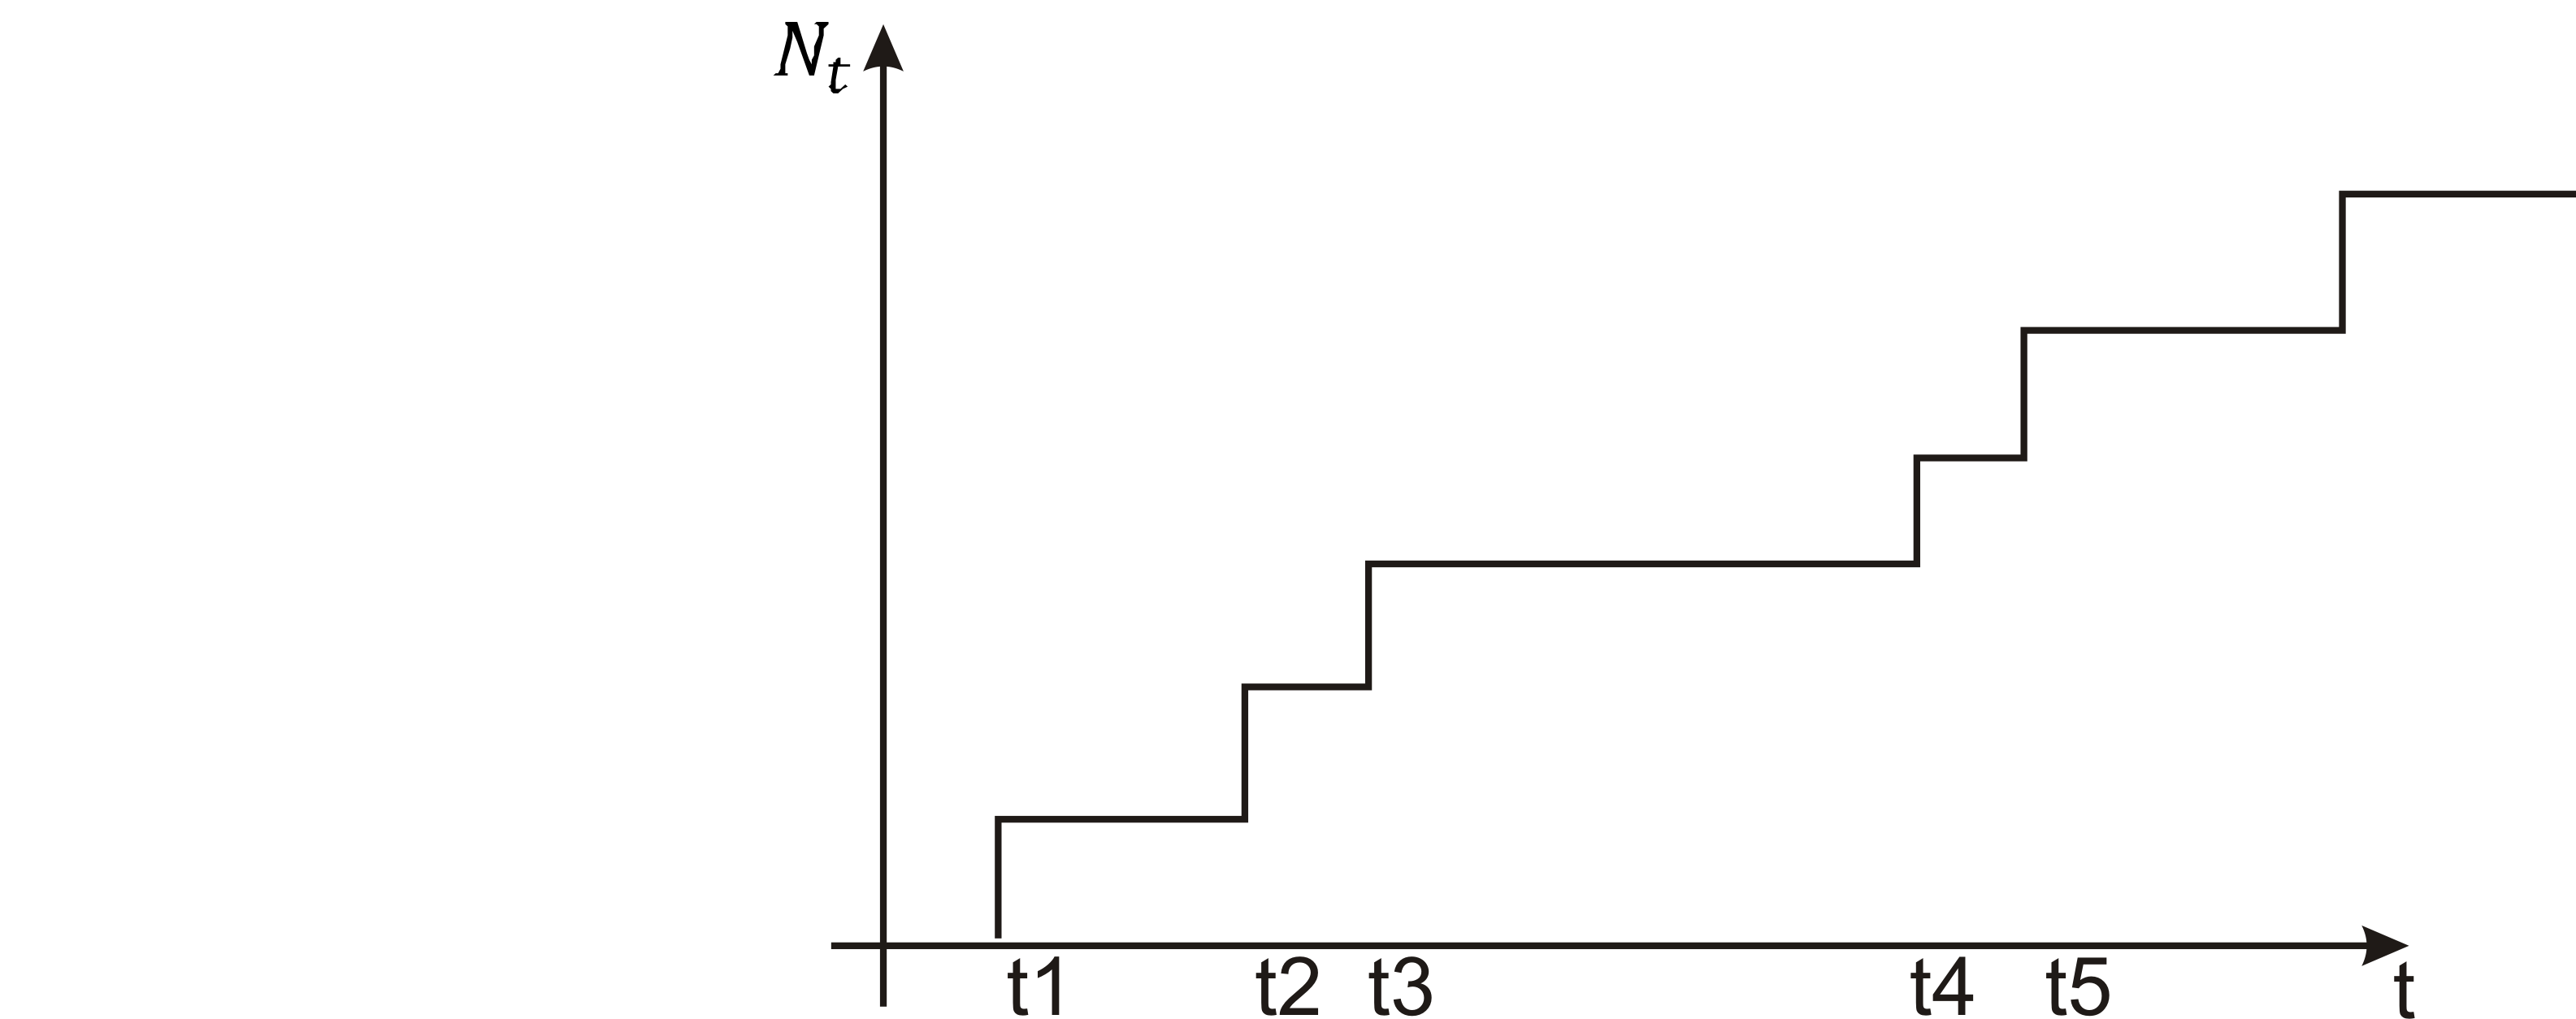
\includegraphics[width=4.5in]{Figures/distr.PNG}\\
 %% \caption{}\label{}
%\end{figure}
The stationary, independent increment property of the probabilistically filtered processes $\{N_1(t), t \geqslant 0\}$ and $\{N_2(t), t \geqslant 0\}$ can be understood and argued out from the example given in the figure. Notice that 
\begin{align*}
	\{N_1(t)=k\} = \bigcup_{n=k}^\infty\{N(t) = n, N_1(t) = k\}.
\end{align*}
Further notice that conditioned on $\{N(t) = n\}$, probability of event $\{N_1(t) = k\}$ is merely probability of selecting $k$ arrivals out of $n$, each with independent probability $p$. Therefore, 
\begin{align*}
	\Pr\{N_1(t)=k\} &= \exp(-\lambda t)\sum_{n=k}^\infty\frac{(\lambda t)^n}{n!}\binom{n}{k}p^k(1-p)^{n-k},\\
	&= \exp(-\lambda t)\frac{(\lambda p t)^k}{k!}\sum_{n=k}^\infty\frac{(\lambda(1-p)t)^{n-k}}{(n-k)!}.% = \exp(-p\lambda t)\frac{(p\lambda t)^k}{k!}.
\end{align*}
Recognizing that infinite sum in RHS adds up $\exp(\lambda(1-p)t)$, the result follows. We can find the distribution of $N_2(t)$ by similar arguments. We will show that events $\{N_1(t) = n_1\}$ and $\{N_2(t) = n_2\}$ are independent. To this end, we see that 
\begin{align*}
	\{N_1(t) = n_1, N_2(t) = n_2\} = \{N(t) = n_1 + n_2, N_1(t) = n_1\}.
\end{align*}
Using their distribution for $N_1(t), N_2(t)$, and conditional distribution of $N_1(t)$ on $N(t)$, we can show that
\begin{align*}
	\Pr\{N_1(t) = n_1, N_2(t) = n_2\} &= \exp(-\lambda t)\frac{(\lambda t)^{n_1 + n_2}}{(n_1 + n_2)!}\binom{n_1 + n_2}{n_1}p^{n_1}(1-p)^{n_2},\\
	&= \Pr\{N_1(t) = n_1\}\Pr\{N_2(t) = n_2\} .
\end{align*}


  %\begin{eqnarray*}
  %% \nonumber to remove numbering (before each align)
    %\Pr\{N_{1}(t) =n]&=& \sum^{\infty}_{m=0}\Pr\{N(t)=m, N_{1}(t) = n]  \\
   %&=& \sum^{\infty}_{m=n}\Pr\{N(t)=m] p^{n}(i-p)^{m-n}mC_n\\
   %&=&  \sum^{\infty}_{m=n}\frac{e^{-\lambda t(\lambda t)^{m}}}{m!}p^{n}(1-p)^{m-n}(mC_n)\\
     %&=& e^{-\lambda t}p^{n}\sum_{m=n}\frac{(\lambda t)^{m-n}}{m!}\frac{(1-p)^{m-n}m!}{n!(m-n)!} \\
     %&=& \frac{e^{-\lambda t p}(p \lambda t)^{n}}{n!} \sum^{\infty}_{m=n}e^{-\lambda (1-p)t}\frac{(\lambda (1-p)t)^{m-n}}{(m-n)!} \\
     %&=&  \frac{e^{-\lambda t p}(p \lambda t)^{n}}{n!} \sum^{\infty}_{k=0}e^{-\lambda (1-p)t}\frac{(\lambda (1-p)t)^{k}}{k!}  \\
     %&=& \frac{e^{-\lambda p t}(p \lambda t)^{n}}{n!}.
  %\end{eqnarray*}
%To show that 
%\begin{eqnarray*}
%% \nonumber to remove numbering (before each align)
   %\{N_{1}(t), t \geq 0\}&\perp&\{N_{2}(t), t \geq 0\}  \\
   %\Pr\{N_{1}(t)&=&n_{1}, N_{2}(t) = n_{2}]\\
    %\Pr\{N(t) = n_{1}+ n_{2}]&=& \frac{e^{-\lambda t} (\lambda t)^{n_{1}+n_{2}}}{(n_{1}+n_{2})!} \\
   %&=&  \frac{e^{-\lambda p t}e^{-\lambda (1-p)t}}{(n_{1}+n_{2})!} -(\lambda t)^{n_{1}+n_{2}}\\
   %&=&  \frac{e^{-\lambda p t}e^{-\lambda (1-p)t} (\lambda t)^{n_{1}}(\lambda t)^{n_{2}}}{n_{1}! n_{2}!}
%\end{eqnarray*}
In general, we need to show finite dimensional distributions factorize. That is, we need to show that for measurable sets $A_1, \hdots, A_n: j \in [m]\}$, we have \begin{align*}
   \Pr\left(\bigcap_{i=1}^n\{N_{1}(t_{i})\in A_{i}\}\bigcap_{j=1}^m\{N_{2}(s_{j})\in B_{j}\}\right)
   =\Pr\left(\bigcap_{i=1}^n\{N_{1}(t_{i})\in A_{i}\}\right)\Pr\left(\bigcap_{j=1}^m\{N_{2}(s_{j})\in B_{j}\}\right).
\end{align*}
\end{proof}
\end{document}